%%%%%%%%%%%%%%%%%%%%%%%%%%%%%%%%%%%%%%%%%%%%%%%%%%%%%%%%%%%%%%%%%%%%%%%%%%%%%%%%
% data_set.tex:
%%%%%%%%%%%%%%%%%%%%%%%%%%%%%%%%%%%%%%%%%%%%%%%%%%%%%%%%%%%%%%%%%%%%%%%%%%%%%%%%
\chapter{Background Estimation}
\label{sec:backgroundEstimation}
%%%%%%%%%%%%%%%%%%%%%%%%%%%%%%%%%%%%%%%%%%%%%%%%%%%%%%%%%%%%%%%%%%%%%%%%%%%%%%%%
The online and offline event selection criteria were applied to the data to select events where two leptons and jets were 
reconstructed, and had kinematics consistent with $\WR \rightarrow \ell\ell jj$ decay progeny.  However, applying these 
selection criteria also selected data events produced by ST background interactions like $\DY$+jets.  
The contribution of ST backgrounds to the $\Mlljj$ distribution found in the data were predicted using Monte Carlo (\MC) 
simulations, and control regions with no \WR signal contamination.  The magnitudes of individual backgrounds, how 
they were simulated, and how the control regions were used to estimate the background contributions are described here.

The magnitude of the background produced by each ST interaction is proportional to its cross section $\times$ branching fraction 
to $\ell\ell jj$ final states in 2015 collisions.  The \DY interaction (Figure \ref{fig:dyDiags}) produced two same flavor 
leptons with a cross section $\times$ branching ratio that peaked at 6000 pb for dilepton mass $\Mll \approx 90$ $\GeV$, 
and decreased rapidly for higher $\Mll$.  At $\sqrt{s} = 13$ $\TeV$ either quark that participates in the \DY interaction 
radiates a parton with a probability of $\sim$0.1, equal to the QCD coupling $\alpha_{QCD}$.  Thus, in $\alpha_{QCD}^{2} \sim$
0.01 $=$1\% of \DY interactions the initial quarks radiate two partons before interacting, and those partons hadronize into 
jets.  Unlike \DY, the $t\bar{t}$ quark interaction (Figure \ref{fig:ttbarDiag}) produced $\ell\ell jj$ final states without 
initial state parton radiation.  Its cross section $\times$ branching ratio, 86 pb, is similar to the 60 pb cross section $\times$ 
branching ratio of \DY$\plus$2 jets.  More than 99\% of top quarks decay to a $W$ boson and bottom quark, so single top quark 
$\plus$ $W$ boson interactions (Figure \ref{fig:singleTopDiags}) produced two leptons and one jet when both $W$ bosons decayed 
leptonically.  The gluon that initiates the top+W interaction radiates a gluon with $\sim$100\% probability, so the top+W interaction 
produced two lepton and two jet final states with a cross section $\times$ branching ratio of $\sim$7 pb.  Other single top quark 
interactions (Figure \ref{fig:singleTopDiags}) produce only one $W$, and therefore did not produce $\ell\ell jj$ final states 
at leading order in the electroweak coupling.  The only other interactions that produce two 
leptons and jets without initial state parton radiation are the WZ and ZZ interactions.  The WZ interaction produces two leptons and 
jets when the $W$ decays hadronically, and the $Z$ decays to charged leptons.  The ZZ interaction produces two leptons and jets 
when one $Z$ decays hadronically, and the other decays to charged leptons.  The combined WZ and ZZ interactions produced $\ell\ell jj$ 
final states in the detector with a cross section $\times$ branching ratio of $\sim$3 pb, negligible compared to the $\DY$+jets 
and $t\bar{t}$ backgrounds.  The WW interaction produces two charged leptons when both $W$ bosons decay leptonically.  The two 
quarks that initiate the WW interaction radiate two partons with $\sim$1\% probability, so the WW interaction produced $\ell\ell jj$ 
final states with a cross section $\times$ branching ratio of $\sim$0.1 pb, negligible compared to other backgrounds.  Although 
the $W$+jets and QCD multi-jet interactions do not produce $\ell\ell$ final states at leading order in the electroweak coupling, 
a small fraction of their jets, less than 0.1\%, were incorrectly reconstructed as charged leptons.  Since the $W$+jets and QCD 
multi-jet interactions produced multiple jets with large cross sections $\times$ branching ratios - in excess of several hundred pb 
\cite{wJetsMeas,jetProductionMeas} - they contributed to the $\Mlljj$ distribution found in data, but at a negligible level.  
In conclusion, the $\DY$+jets and top quark interactions produced the largest backgrounds, and other interactions produced negligible 
backgrounds.  The shape and magnitude of the $\Mlljj$ distribution produced by these interactions was estimated using Monte Carlo 
(\MC) simulations.

\begin{figure}[btp]
	\centering
	\subfigure{
		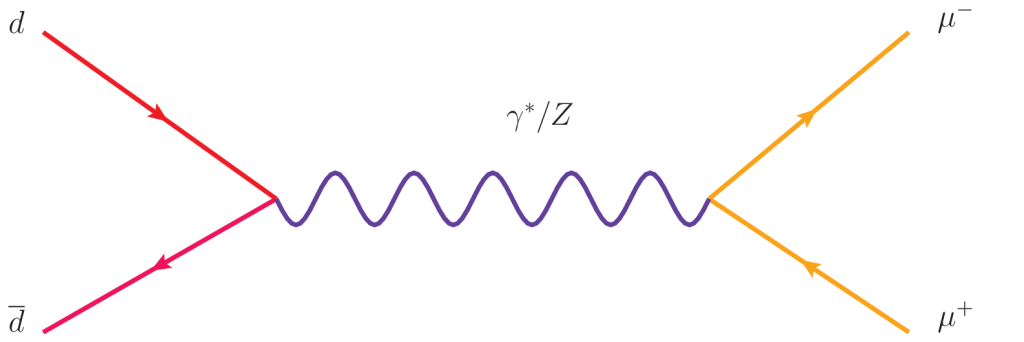
\includegraphics[width=0.45\textwidth]{figures/dyNoJetFeynDiagram.png}
	}
	\subfigure{
		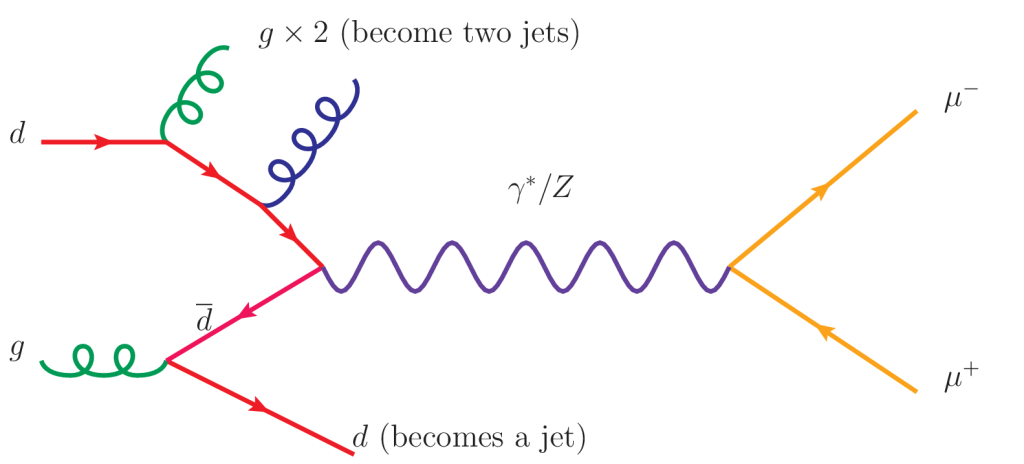
\includegraphics[width=0.45\textwidth]{figures/dyThreeJetFeynDiagram.png}
	}
	\label{fig:dyDiags}
	\caption{Feynman diagrams for the \DY interaction with 0 radiated partons, and 3 radiated partons \cite{dyDiagrams}.}
\end{figure}

\begin{figure}[h]
	\centering
	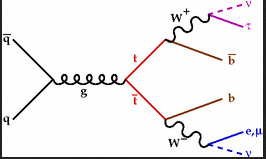
\includegraphics[width=0.7\textwidth]{figures/topAntiTopFeynDiagram.png}
	\caption{$t\bar{t}$ Feynman diagram \cite{ttbarDiagram}.}
	\label{fig:ttbarDiag}
\end{figure}

\begin{figure}[h]
	\centering
	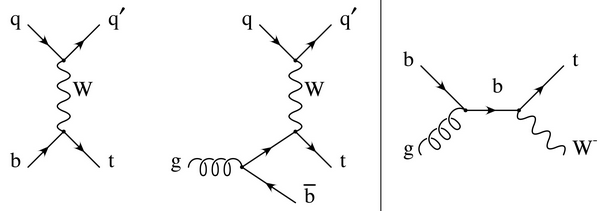
\includegraphics[width=0.7\textwidth]{figures/singleTopQuarkFeynDiagrams.png}
	\caption{Single top quark Feynman diagrams \cite{singleTopQrkDiagrams}.}
	\label{fig:singleTopDiags}
\end{figure}


\section{Monte Carlo}
\label{sec:MC}
%Events from \WR processes, characterized by different \mnul and \mWR, and backgrounds are simulated in three steps.
%\PYTHIA also provides a flexible, generic \WR signal model that is based on the ST weak interaction model; for this reason \PYTHIA 
%was also used to simulate $\WR \rightarrow \ell\ell jj$ interactions.  
Background events are simulated in three steps.  The first 
step simulates the interaction between colliding protons, the decay of unstable particles, and the hadronization of 
partons leaving the interaction with one or two \MC generators.  For particles produced in the first step that interact with 
any sub-detector, the second step simulates the electronic signals generated in each sub-detector.  In the third step, the 
reconstruction algorithms process these signals to reconstruct leptons and jets.

In the first step one \MC generator simulates the interaction between colliding protons, and the decay of unstable particles.  
The \MC generator used to simulate the each background was chosen to match the strengths of the generator 
with the characteristics of the interaction.  The \MADGRAPH generator \cite{madgraph} simulates all Feynman diagrams of a 
interaction at leading order in the electroweak coupling with up to 4 additional partons radiated from the interaction.  Due to the 
$\alpha_{QCD}$ cross section penalty of radiating an additional parton, 
simulating up to 4 radiated partons was only warranted for high cross section $\times$ branching ratio interactions - \DY, 
$t\bar{t} \rightarrow \ell\ell jj$, and $W \rightarrow \ell\nu$.  Therefore, \MADGRAPH was used to simulate the $\DY$+jets, $t\bar{t}$ 
and $W$+jets interactions.  In contrast with \MADGRAPH, the \POWHEG generator \cite{powheg} simulated all Feynman diagrams of a 
interaction at next-to-leading order in the electroweak and QCD couplings with up to one additional parton radiated from the interaction.  
\POWHEG was used to simulate single top quark interactions because their cross sections $\times$ branching ratios to $\ell\ell jj$ 
final states are at least 7\% larger at next-to-leading order relative to leading order \cite{singleTopNLOvsLO}.  
Although the next-to-leading order correction to the diboson (WW, WZ, ZZ) cross section $\times$ branching ratio was up to 45\% 
\cite{dibosonLOvsNLO}, the diboson background is still negligible compared to the $\DY$+jets and top quark backgrounds.  Therefore, 
the production and decay of diboson pairs was simulated using the leading order \PYTHIA generator \cite{pythia8,Sjostrand:2006za}, 
with up to one additional parton radiated from the interaction.  Events simulated with any \MC generator show the best agreement with 
experimental data when \PYTHIA is used to simulate parton hadronization \cite{pythiaForHadronization}, so all simulations used \PYTHIA 
and the NNPDF23 PDF set \cite{nnpdf} to hadronize partons.  Excluding the partons, the \MC generator that simulated the pp interaction 
also simulated the decays of unstable particles to quasi-stable and stable particles, like the $\Sigma^{\pm}$ and $\gamma$, that travel 
a mean distance c$\tau \gtrsim 2.4$ cm before decaying.  Particles that travel a mean distance of 2.4 cm have a small probability 
to interact with the first silicon pixel tracker layer located 4.4 cm from the interaction point \cite{cmsTdrPhysPerformance}, so they 
are included in the second simulation step.

%SAVE THIS statement that explains why the aMCatNLO inclusive diboson simulated datasets were not used
%A second set of diboson$\to$leptons+jets events was simulated with a next-to-leading order \MC generator, but these events were 
%generated with positive and negative event weights.  Due to the presence of positive and negative event weights, in some $\Mlljj$ 
%regions the predicted number of diboson events was negative, and the prediction's statistical uncertainty was greater than 100\%.

In the second step the effect of pileup is simulated, and GEANT \cite{geant4} simulates the propagation and decay of 
quasi-stable and stable particles, and their interactions with the CMS detector.  The large instantaneous luminosity of the LHC 
beams produced multiple pp interactions, pileup, in each selected data event.  When \MC simulations started in the spring of 2015, 
the pileup distribution in data was expected to follow a Poisson distribution with mean 12.  In each event produced 
by the first step, the effect of pileup is simulated by pulling a 
random integer $X$ from a Poisson distribution with mean 12, and mixing $X$ simulated minimum bias events into the event.  The 
minimum bias events were simulated only through the first simulation step.  \PYTHIA simulates minimum bias events whose reconstructed 
particle kinematics show the best agreement with particles reconstructed in minimum bias events in data \cite{pythiaForHadronization}, 
so \PYTHIA was used to simulate minimum bias events.  After adding minimum bias events to simulate pileup, GEANT propagates all particles 
(stable and quasi-stable) in the 3.8 $\unit{T}$ magnetic field, simulates their interactions with the detector, and simulates the decays 
of quasi-stable particles to stable particles - $\gamma,p^{\pm},n^{0},\bar{n}^{0},\nu,e^{\pm}$.  Finally, for particles that interact 
with the detector, GEANT simulates the signal generated in the detector.

In the third step the online trigger and offline reconstruction algorithms process the detector signals simulated by GEANT.  The 
final decision of each trigger algorithm, to keep or discard the event, is saved in each simulated event, but no events are discarded 
for any reason.  Then, the same offline reconstruction algorithms used in real collisions are used to reconstruct interaction vertices, 
leptons, and jets.

After finishing the third simulation step, particle energy corrections and event weights were applied to simulated events.  As 
explained previously, the energies of simulated jets, muons, and electrons were corrected to match the energy of particles 
reconstructed in data.  The differences in lepton reconstruction, trigger selection, and offline ID selection efficiencies between 
data and simulated events were corrected by changing the weight of each simulated event, up to $\pm$7\%, depending on the $\pt$ and 
$\eta$ of the selected leptons.  Independent of the reconstructed particle kinematics, the weight of each simulated event 
was normalized to the integrated luminosity of the data, and adjusted further to match the pileup distribution found in the data.  The 
simulated pileup distribution is a Poisson distribution with mean 12, but the pileup distribution found in the data is better 
represented by a Poisson distribution with mean 14 \cite{lumi}.  The discrepancy between the data and simulated pileup distributions 
was corrected by changing the weight of each simulated event, on average by $\sim$5\%.

The simulated interactions are summarized in Table \ref{tab:centrallyProducedMC}.  The number of simulated events are expressed in units 
of integrated luminosity, and should be compared to the 2.6 fb$^{-1}$ of data \cite{lumi}.

\begin{table}[bt]
	\caption{The ST background and \WR signal (only $\mnul = \frac{1}{2}\mWR$) simulated datasets.  The "Size" of a dataset is equal 
	to the number of simulated events divided by the 13 $\TeV$ cross section $\times$ branching fraction of the process.}
\label{tab:centrallyProducedMC}

\centering
\resizebox{\textwidth}{!}{
	\begin{tabular}{ |c|c|c|c| } 
	\hline
	Dataset         & Step 1 Generator & cross section (pb) & Size (fb$^{-1}$)   \\
		\hline
		Inclusive DY+jets, $DY \rightarrow ll$ & \MADGRAPH   & 5991    & 1.51 \\ \hline
		DY+jets HT 100-200, $DY \rightarrow ll$ & \MADGRAPH   & 181.3    & 15.0 \\ \hline
		DY+jets HT 200-400, $DY \rightarrow ll$ & \MADGRAPH   & 50.42    & 19.3 \\ \hline
		DY+jets HT 400-600, $DY \rightarrow ll$ & \MADGRAPH   & 6.984    & 153. \\ \hline
		DY+jets HT $>$ 600, $DY \rightarrow ll$ & \MADGRAPH   & 2.704    & 369. \\ \hline
		t$\bar{t}$+jets $\rightarrow ll$+jets & \MADGRAPH  & 85.67    & 286. \\ \hline
		single t $\rightarrow$ leptons+jets  & \POWHEG & 80.95 & 20.8 \\ \hline
		single $\bar{t}$ $\rightarrow$ leptons+jets & \POWHEG & 136.0 & 24.3 \\ \hline
		$\bar{t}$+W $\rightarrow$ all   & \POWHEG & 35.85 & 27.6 \\ \hline
		t+W $\rightarrow$ all   & \POWHEG & 35.85 & 27.8 \\ \hline
		WW $\rightarrow$ all  & \PYTHIA & 113.8   & 8.73   \\ \hline
		ZZ $\rightarrow$ all  & \PYTHIA & 10.15   & 98.2   \\ \hline
		WZ $\rightarrow$ all  & \PYTHIA & 23.4   & 41.8   \\ \hline
		W+jets $\rightarrow l\nu$+jets & \MADGRAPH & 50270   & 1.44 \\ \hline
		$\WR \rightarrow l\nul \rightarrow lljj$  & \PYTHIA & 1$\times 10^{-5}$ - 4.3 & 5$\times 10^{6}$ - 11.6   \\ \hline
		\end{tabular}
}
\end{table}

%MOVE information about WR signal events into appendix on WR signal MC
Two sets of \WR signal events were simulated using \PYTHIA - one set was simulated through all three simulation steps, the other 
was simulated through the first step.  The set simulated through all three steps was produced with \mWR stepping from 0.8 to 6 
$\TeV$ in increments of 0.2 $\TeV$, and $\mnul = \frac{1}{2}\mWR$; these fully reconstructed events are used to calculate cross 
section $\times$ branching ratio limits on the $\WR \rightarrow \ell\ell jj$ process as a function of \mWR.  The other set was 
produced with \mWR stepping from 0.8 to 4.0 $\TeV$ in increments of 0.1 $\TeV$, and, at each \mWR, several \mnul values between 
$0.1 \leq \mnul < \mWR$ $\TeV$.  If no \WR signal is found, these events are used to set \mWR and \mnul exclusion limits for 
$\mnul \neq \frac{1}{2}\mWR$.


\section{Top Quark Background}
\label{sec:topQrkBkgnds}
Top quark interactions, primarily $t\bar{t}$ production, produce bottom quarks that hadronize into jets, and $W$ bosons that 
decay into charged leptons.  Since $W$ bosons decay to electrons and muons with equal branching fractions, top quark interactions 
produce the $e\mu jj$ final state twice as often as the $eejj$ or $\mu\mu jj$ final states.  The $e\mu jj$ final state is not 
contaminated with \WR signal (Chapter \ref{sec:lrsPhenomenology}) or other background interactions, so the $e\mu jj$ final state was 
used as a control region to estimate the top quark background.  During collisions, $e\mu jj$ events were selected using the 
Level-1 single muon trigger described in Chapter \ref{sec:muOnlineSel}.  Then, events were required to pass the following $e\mu$ HLT 
selection criteria:

\begin{itemize}
	\item A track reconstructed in the silicon tracker with $\pt > 30$ $\GeV$ and $|\eta| < 2.4$ was geometrically matched to 
		the muon detector track segment that passed the L1 trigger.
	\item In the plane perpendicular to the beam axis, the distance between the silicon tracker track origin and its 
		reconstructed vertex was $< 1$ mm.
	\item One 5 $\times$ 5 ECAL crystal cluster was required to have $\Et > 30$ $\GeV$.
	\item For the selected ECAL cluster (energy E):
	\begin{itemize}
		\item The hadronic energy behind the cluster was $<$ 15\% of E in the barrel, and $<$ 10\% of E in the endcap. 
		\item Ninety percent of E was measured in an area that was two crystals wide in $\eta$.
		\item If the cluster was in the barrel, a reconstructed track with signals in at least two pixel tracker layers 
			extrapolated close to the cluster position.  The track extrapolated from the pixel tracker to within $2.3$ cm 
			of the cluster $z$ position, and to within 1 ECAL crystal area of the cluster $(\eta,\phi)$ position.
	\end{itemize}
\end{itemize}

In selected events, muons, electrons, and jets were reconstructed and selected using the reconstruction algorithms and selection 
criteria described in Chapter \ref{sec:reco_chapter}.  The same selection criteria were applied to simulated background events, and compared 
to the selected data events in Figure \ref{fig:dataAndSimsInEMuChannel}.  Comparing the magnitudes of different simulated backgrounds, the 
top quark background produces more than 98\% of selected $e\mu jj$ events as expected.

\begin{figure}[h]
	\centering
	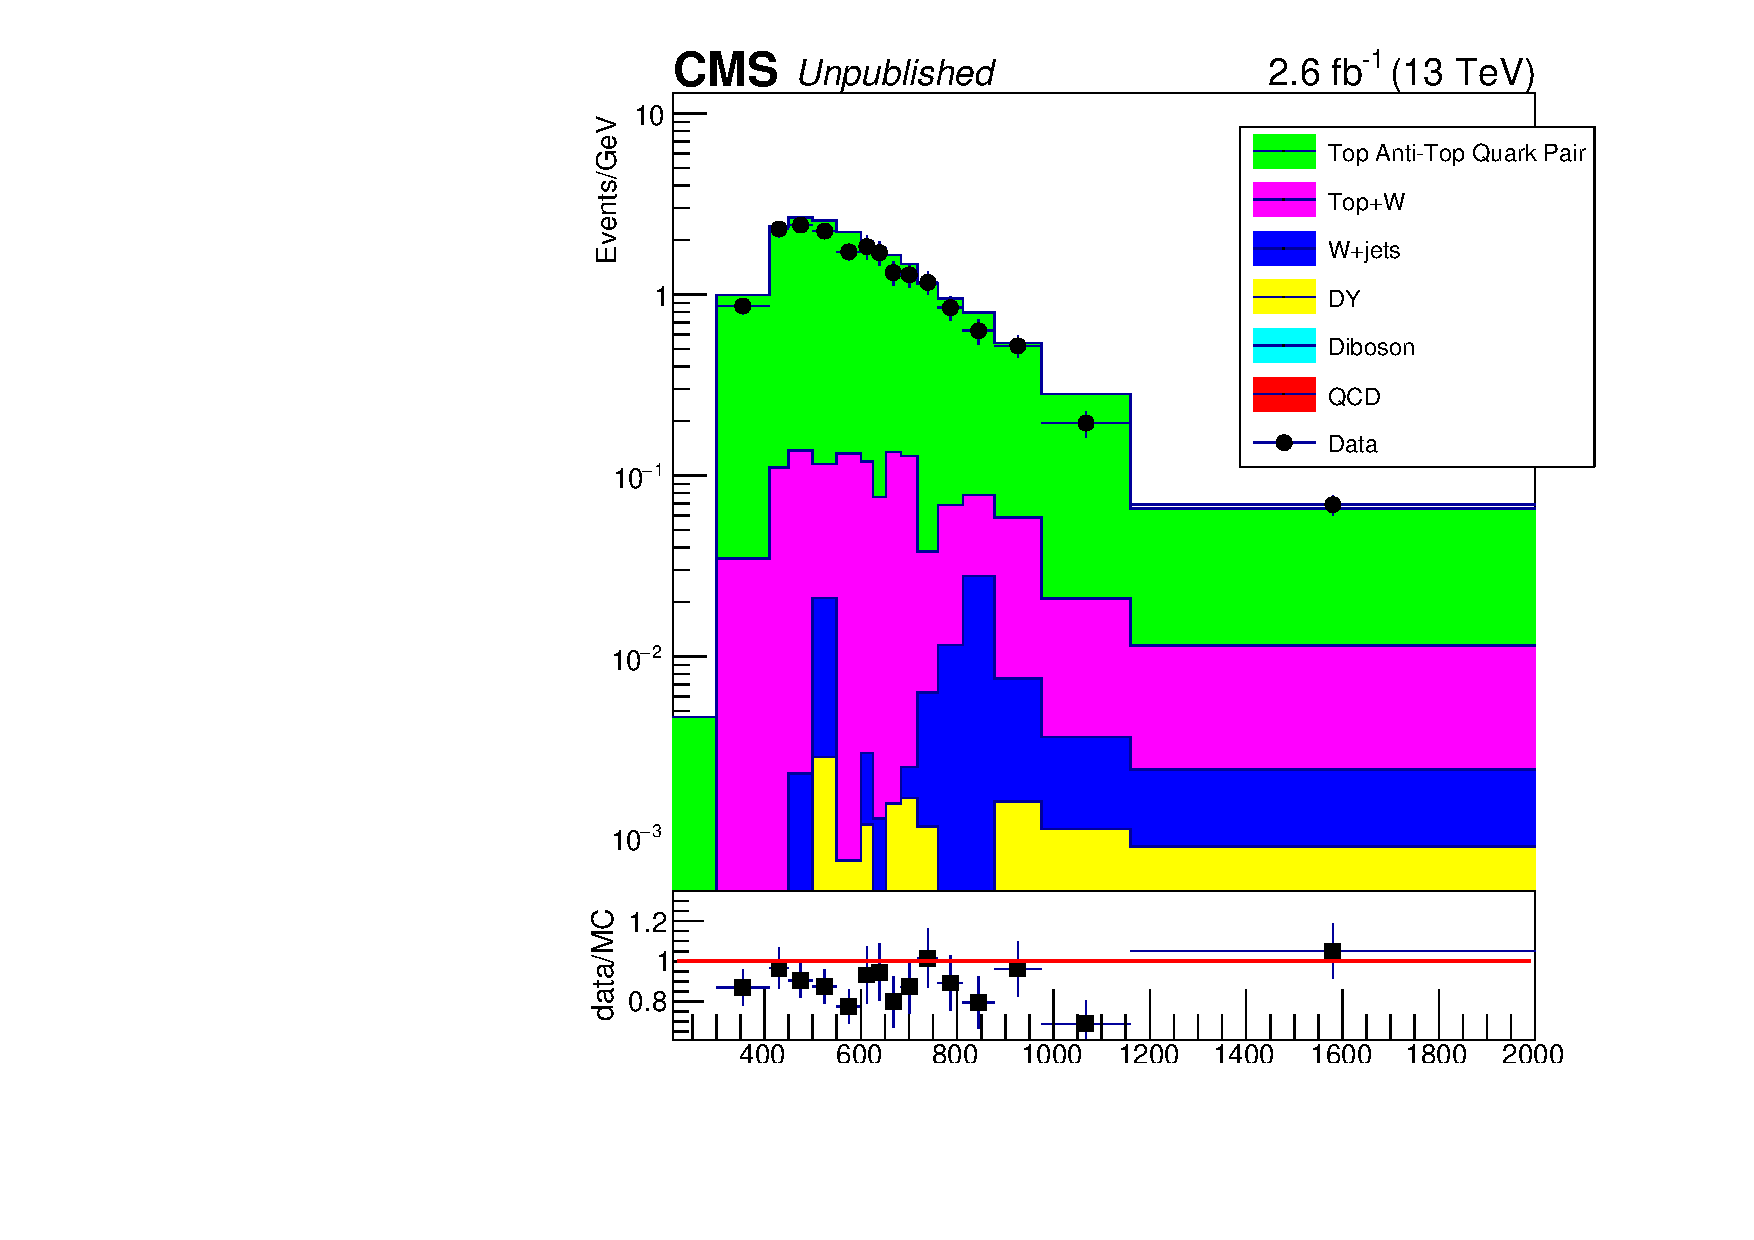
\includegraphics[width=0.7\textwidth]{figures/Mlljj_eMuChannel_log.pdf}
	\caption{The $\Mlljj$ distribution from data and simulated ST events that passed the $e\mu$ selection criteria, excluding 
	the $\Mlljj > 600 \GeV$ cut.  The bin widths were variable, and their contents were normalized to the bin widths.}
	\label{fig:dataAndSimsInEMuChannel}
\end{figure}

The $\Memujj$ distribution found in selected data events was scaled by two factors to estimate the top quark background in the $ee$- 
and $\mu\mu$-channels.  The first factor - the ratio of $\ell\ell / e\mu$ production - is 0.5, and is independent of $\Mlljj$.  The 
second factor - the ratio of electron to muon selection efficiency $\frac{e}{\mu}$ - is expected to be below 1 because electrons are 
not reconstructed in the ECAL barrel-endcap transition region $1.44 < |\eta| < 1.57$.  However, the exact value of $\frac{e}{\mu}$ and 
its variation with $\Mlljj$ were not known a priori.  The product of the two factors and its variation with $\Mlljj$ was estimated using 
simulated top quark background events.  First, simulated events were selected using the $e\mu$-, $ee$-, and $\mu\mu$-channel selection 
criteria.  Then, the $\Mlljj$ distributions found in each set of events were split into variable width bins such that each bin had 
the same number of events.  The first bin covered $600 < \Mlljj \leq 625$ $\GeV$, and the last bin covered $\Mlljj > 1160$ $\GeV$.  
Then the integral of each bin was calculated for all three distributions.  Finally, the integrals of the $\Meejj$ and $\Mmumujj$ bins 
were divided by the integrals of the $\Memujj$ bins.  The result, shown in Figure \ref{fig:ttbarSFratios}, represents the product of 
the $\ell\ell / e\mu$ production ratio and the $\frac{e}{\mu}$ or $\frac{\mu}{e}$ selection efficiency ratio as a function of $\Mlljj$.  
The result within statistical uncertainty is consistent with a constant value versus $\Mlljj$: 0.659 for $\Mmumujj / \Memujj$, 0.432 
for $\Meejj / \Memujj$.  This confirms that the $\Mlljj$ distribution shape found in top quark events is independent of the final state 
lepton flavor.  Furthermore, the $\Memujj$ distribution found in data is related by a multiplicative constant to the $\Meejj$ and 
$\Mmumujj$ distributions found in data that were produced by top quark interactions.

\begin{figure}[btp]
	\centering
	\subfigure{
		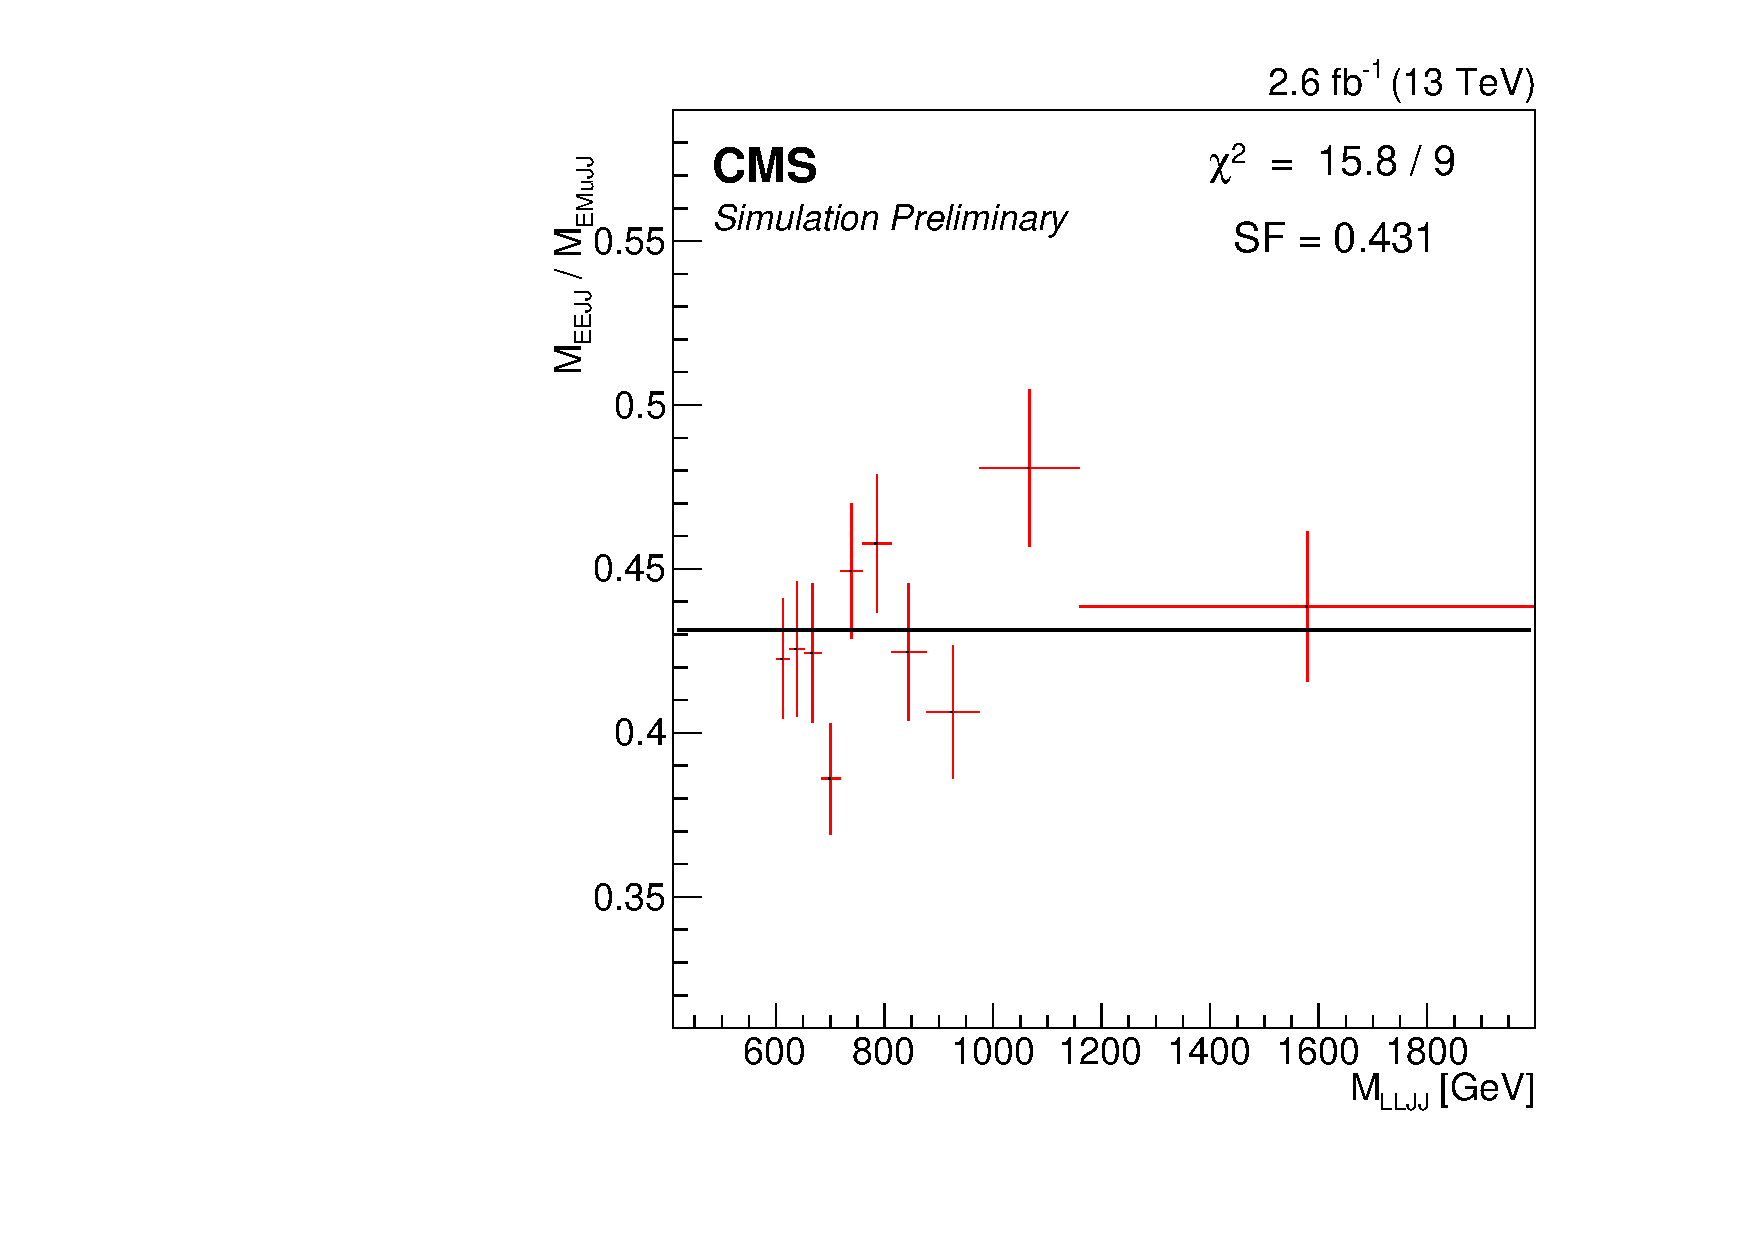
\includegraphics[width=0.45\textwidth]{figures/flavor_ratio_EE_variablebinwidth.pdf}
	}
	\subfigure{
		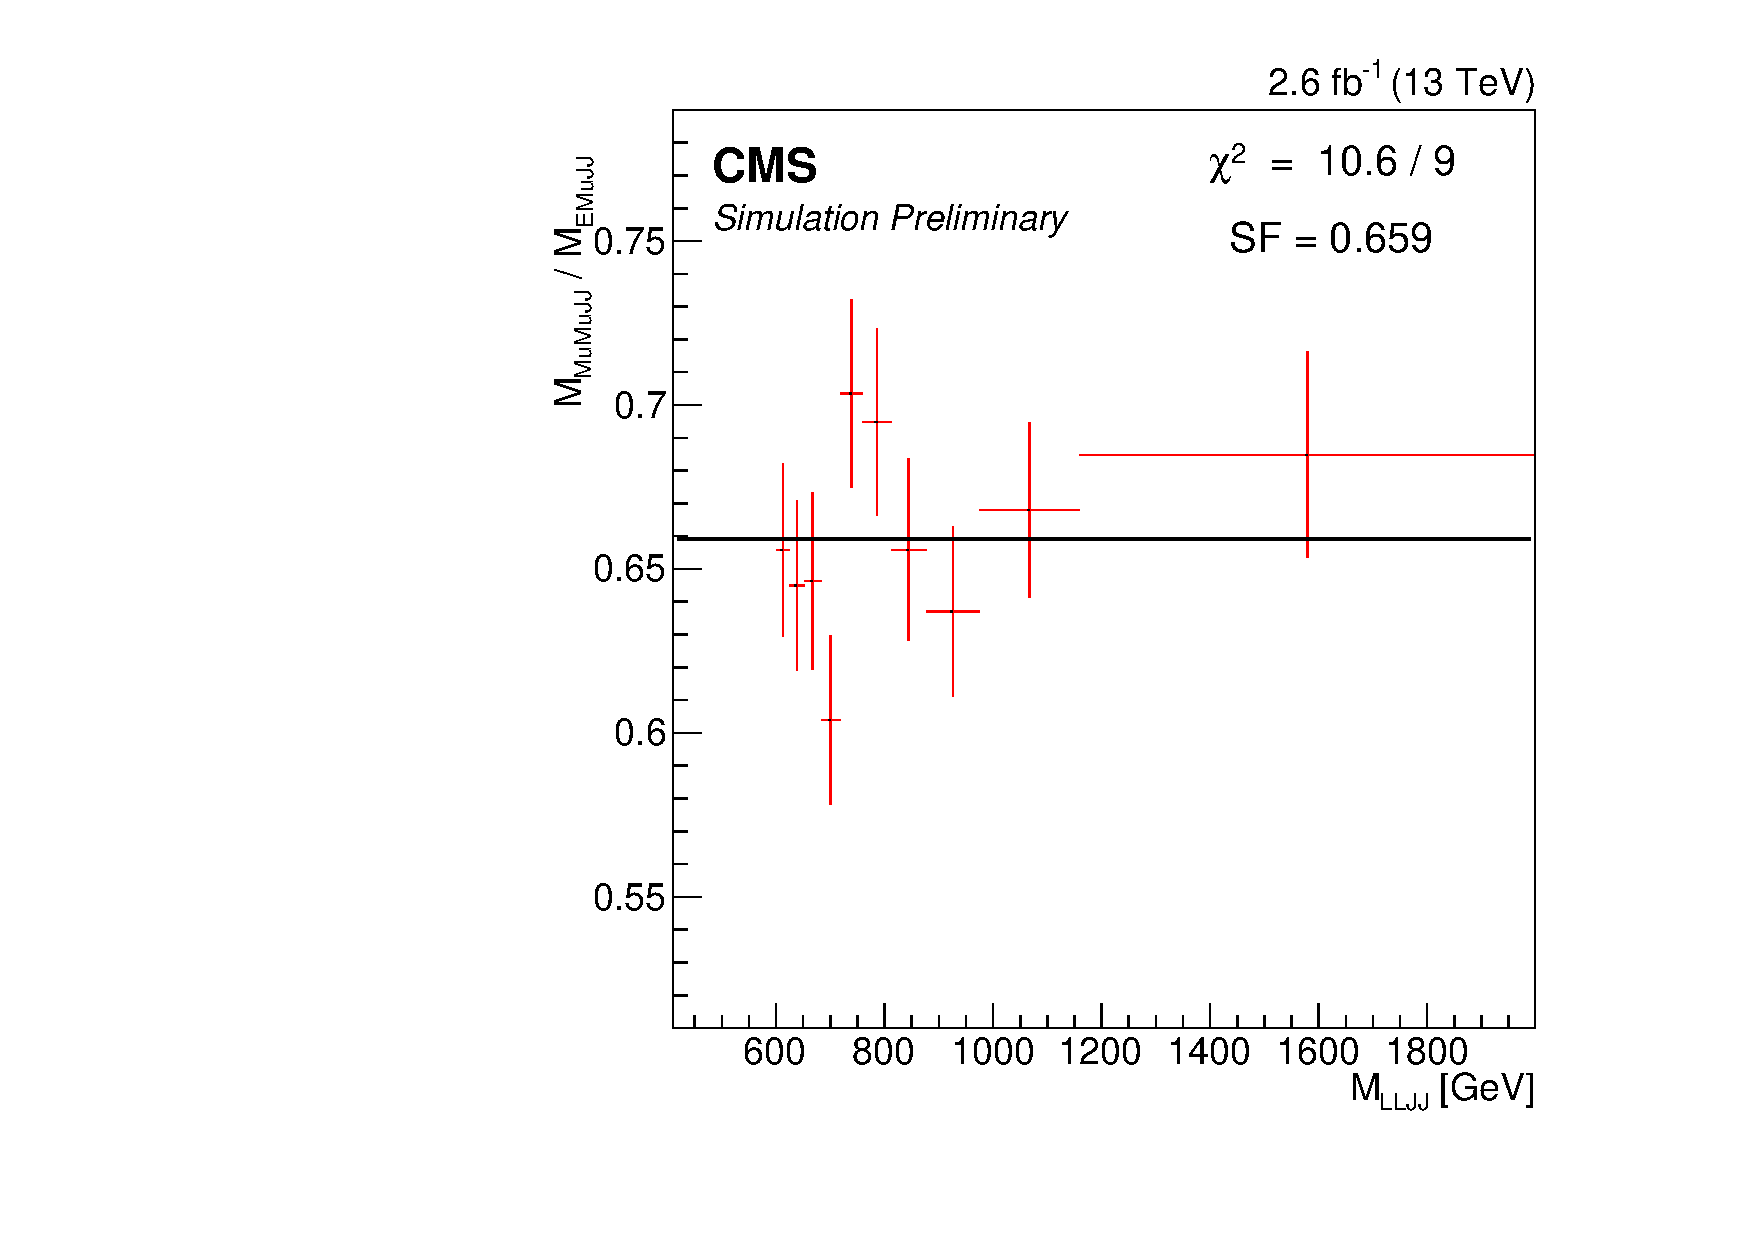
\includegraphics[width=0.45\textwidth]{figures/flavor_ratio_MuMu_variablebinwidth.pdf}
	}
	\label{fig:ttbarSFratios}
	\caption{The bin-by-bin ratio of the $\Mlljj$ and $\Memujj$ distributions from simulated top quark backgrounds, where 
		$\ell$ is an electron on the left, and a muon on the right.}
\end{figure}

The $\Memujj$ distribution found in data was multiplied by 0.659 or 0.432 to estimate the top quark $\Mlljj$ distribution in the 
$\mu\mu$- and $ee$-channel, respectively.  Although the values 0.659 and 0.432 were calculated using all simulated events with 
$\Mlljj > 600$ $\GeV$, few events with $\Mlljj > 1500$ $\GeV$ contributed.  A 10\% uncertainty was assigned to the top quark background 
estimate to cover any deviation from 0.659 or 0.432 at high $\Mlljj$.  Based data and simulated events in Figure 
\ref{fig:dataAndSimsInEMuChannel}, the non-top quark backgrounds contributed $\sim$1\% to the $\Memujj$ distribution found in data.  
Their contribution was neglected because it was small compared to the 10\% top quark background uncertainty.


\section{\DY Background}
\label{sec:dyBkgnd}
The $\DY$+jets interaction produced $\ell\ell jj$ events at a similar rate to the top quark interactions.  The $\Mlljj$ distribution 
produced by the \DY+jets interaction was estimated using simulated \DY+jets events.  Simulated \DY+jets events were selected using 
the $ee$- and $\mu\mu$-channel requirements described previously.  In both channels selected events defined the shape and approximate 
normalization of the $\Mlljj$ distribution, but the normalization was adjusted based on comparisons between simulations and data in 
three control regions.

\subsection{\DY Normalization in $\Mlljj$}
\label{sec:dyNormInMlljj}
$\DY$+jets events were simulated using the \MADGRAPH generator at leading order in the electroweak and strong couplings, while 
$\DY$+jets events observed in data were produced at all orders in these couplings.  The simulated events were normalized to the 
integrated luminosity of data using the simulated cross section $\times$ branching ratio.  Thus, the higher order cross section 
corrections created a \DY normalization discrepancy between simulations and data.

The normalization discrepancy was estimated by comparing data to simulated $\DY$+jets events using the $Z \rightarrow \ell\ell$ control 
region, where the majority of events were produced by $\DY$+jets interactions.  Events in the $ee$-channel control region were selected 
by a Level-1 trigger that required one 5 $\times$ 5 ECAL crystal cluster with $\Et > 30$ $\GeV$ and $|\eta| < 2.1$.  Then, selected 
events were required to pass the following double-electron HLT selection criteria:

\begin{itemize}
	\item One 5 $\times$ 5 ECAL crystal cluster was required to have $\Et > 30$ $\GeV$, and a second non-overlapping cluster 
		was required to have $\Et > 4$ $\GeV$.
	\item For the cluster with $\Et > 30$ $\GeV$ (energy E):
	\begin{itemize}
		\item The hadronic energy behind the cluster was $<$ 5.5\% of E in the barrel, and $<$ 7\% of E in the endcap. 
		\item Ninety percent of E was measured in an area that was two crystals wide in $\eta$.
		\item A reconstructed track with signals in at least two pixel tracker layers extrapolated close to the cluster 
			position.  The track extrapolated from the pixel tracker to within 1 cm of the cluster $z$ position, and to 
			the cluster $(\eta,\phi)$ position within half the area of one ECAL crystal.
		\item The cluster $\Et$ and matching track $\pt$ cannot differ by more than 50\%. 
		
		\item In a $\Delta R =$ 0.3 radius cone centered on the cluster:
		\begin{itemize}
			\item The total ECAL energy not measured in the cluster was $<$ 22.5\% of E in the barrel, and $<$ 12.1\% of 
				E in the endcap.
			\item The total HCAL energy was $<$ 15.5\% of E in the barrel, and $<$ 16\% of E in the endcap.
		\end{itemize}
	\end{itemize}
\end{itemize}

Events in the $\mu\mu$-channel control region were selected by a Level-1 single muon trigger.  The Level-1 trigger was identical to the 
Level-1 single muon trigger described in Chapter \label{sec:topQrkBkgnds}, but required one track to have $\pt > 20$ $\GeV$.  Then, 
selected events were required to pass the following single muon HLT selection criteria:

\begin{itemize}
	\item A track reconstructed in the silicon tracker with $\pt_{1} > 22$ $\GeV$ and $|\eta| < 2.4$ was geometrically matched to 
		the muon detector track segment, reconstructed with $\pt_{2}$ that passed the L1 trigger.
	\item In the plane perpendicular to the beam axis, the distance between the silicon tracker track origin and its 
		reconstructed vertex was $< 1$ mm.
	\item In a $\Delta R =$ 0.3 radius cone centered on the muon trajectory:
		\begin{itemize}
			\item The total ECAL energy was $<$ 11\% of $\pt_{2}$ in the barrel, and $<$ 8\% of $\pt_{2}$ in the endcap.
			\item The total HCAL energy was $<$ 21\% of $\pt_{2}$ in the barrel, and $<$ 22\% of $\pt_{2}$ in the endcap.
			\item The total $\pt$ of all silicon tracker tracks excluding the muon track was $<$ 9\% of $\pt_{1}$.
		\end{itemize}
\end{itemize}

Simulated electrons passed the electron trigger criteria with a different efficiency than leptons produced in real collisions.  This 
efficiency difference was corrected by multiplying the weight of every selected $Z\rightarrow ee$ simulated event by a weight that 
depended on the $\Et$,$\eta$ of the electron with $\Et > 30$ $\GeV$; the average weight was 0.96 (4\% decrease).  Muons in data and 
simulations passed the muon trigger criteria with the same efficiency, so no correction was applied.

In events selected by the triggers, reconstructed leptons and jets were required to pass offline selection criteria.  The ID 
criteria are identical to those described previously, but the kinematic selection criteria, in Table \ref{tab:cutsZllReg}, include 
lower lepton $\pt$ thresholds to select more $Z\rightarrow \ell\ell$ events.

\begin{table}[h]
	\caption{The kinematic selection criteria applied to events in the $Z\rightarrow \ell\ell$ control region 
	to select two leptons and two jets.}
	\label{tab:cutsZllReg}
	\centering
	\begin{tabular}{c|c}
		variable & criteria \\  \hline
		jet $\pt$ and $\eta$ & $\pt > 40$, $|\eta| < 2.4$ \\
		lepton-jet separation & $\Delta R > 0.4$ \\
		lepton $\pt$ and $\eta$ & $\pt > 35$, $|\eta| < 2.4$ \\
		di-lepton mass $\Mll$ & $70 < \Mll < 110$ \\
	\end{tabular}
\end{table}

The $\Mll$ distribution found in selected $Z\rightarrow \ell\ell$ events was compared between data and $\DY$+jets simulations.  Their 
shapes matched, but the normalization of the data events exceeded that of simulated events by 15.7\% in the $ee$-channel, and by 14.2\% 
in the $\mu\mu$-channel.  Therefore, the $\DY$ background normalization was increased by 15.7\% in the $ee$-channel, and by 14.2\% in the 
$\mu\mu$-channel.  The uncertainty on this normalization correction, discussed next, is comparable to the background from top quark and 
other interactions in the $Z \rightarrow \ell\ell$ control region, so the other interactions were neglected.

Two additional $\DY$+jets datasets were simulated using different generators, and used to estimate the uncertainty on the $\sim$15\% 
\DY normalization correction.  Of the two other generators, one simulated the \DY interaction at next-to-leading order in the electroweak 
and QCD couplings with up to four radiated partons leaving the interaction.  \POWHEG, which only simulates up to one radiated parton leaving 
the \DY interaction, was used to produce the other dataset.  Events from data and all three simulated datasets were selected using the 
$Z \rightarrow \ell\ell$ selection criteria without jet requirements.  The jet requirements were removed to compare data to simulations in 
a phase space where \POWHEG yielded a large number of selected events, comparable to the other simulated datasets.  The $\Mll$ distributions 
found in simulated events were compared to the distributions found in data.  Their shapes matched, but the normalization differed between 
data and simulations.  Since the simulations were expected to match the data, the largest normalization difference between any of the three 
simulations and data was taken as the uncertainty on the $\sim$15\% normalization correction.  The uncertainty was 2.0\% in the $ee$-
channel and 1.0\% in the $\mu\mu$-channel.

\subsection{\DY Shape in $\Mlljj$}
\label{sec:dyShapeInMlljj}
$\DY$+jets events were simulated at leading order in the QCD coupling with up to four radiated partons leaving the \DY interaction.  \DY 
interactions in real collisions radiate partons, with no upper limit, through processes at all orders in the QCD coupling.  Therefore, the 
$\pt$,$\eta$, and multiplicity spectra of radiated partons in real and simulated \DY events were not expected to agree.  More than 50\% of 
partons radiated with $|\eta| < 2.5$ and $\pt > 10$ $\GeV$ were reconstructed as jets \cite{pflowEventReco}, so the reconstructed jet $\pt$, 
$\eta$, and multiplicity distributions found in data and simulated events were not expected to agree.  As a result, the shapes of the 
$\Mlljj$ distributions found in real and simulated \DY events were expected to differ.

The size of the $\Mlljj$ distribution shape discrepancy was estimated using the low $\Mll$ control region, where the dominant 
background was $\DY$+jets.  Events from data and all simulated backgrounds in the $ee$- and $\mu\mu$-channel control regions were selected 
using the triggers, offline ID, and offline kinematic selection criteria described in Chapter \ref{sec:reco_chapter}.  However, the 
di-lepton mass cut was changed from $\Mll > 200$ $\GeV$ to $\Mll < 180$ $\GeV$.  The normalization of simulated $\DY$+jets events was 
increased by $\sim$15\%, then the $\Mlljj$ distributions found in selected data and simulated events were compared (Figure 
\ref{fig:mlljjLowMllCR}).  The size of the $\Mlljj$ shape discrepancy was calculated as the largest difference between the data and the 
total estimated background in any bin.  The maximum discrepancy, 40\% for $\Mlljj > 1.9$ $\TeV$ in both channels, was conservatively 
taken as the shape discrepancy for all simulated $\DY$+jets events that had $\Mlljj > 0.6$ $\TeV$.

\begin{figure}[btp]
\centering
\subfigure{
  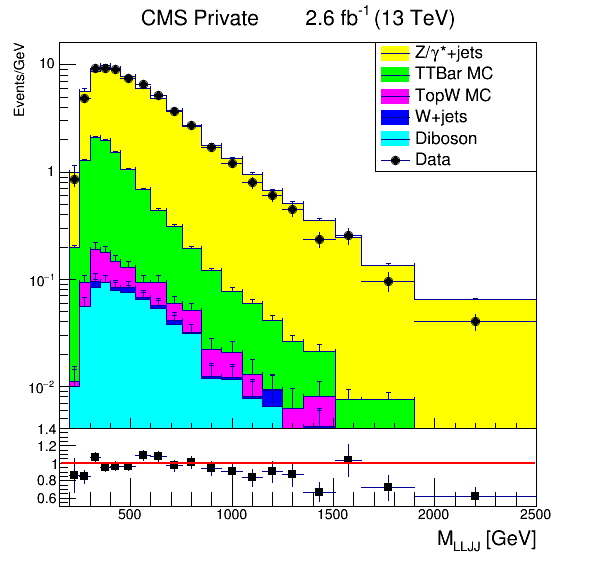
\includegraphics[width=0.45\textwidth]{figures/Mlljj_eeChnl_lowMllCR.png}
}
\subfigure{
  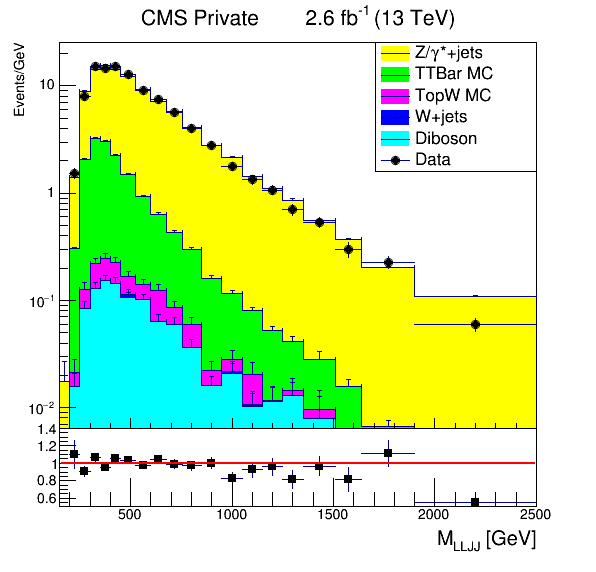
\includegraphics[width=0.45\textwidth]{figures/Mlljj_mumuChnl_lowMllCR.png}
}
\caption{The $\Mlljj$ distributions from data and simulated ST background events that passed the low $\Mll$ region selection criteria.  
	The $ee$-channel is on the left, and the $\mu\mu$-channel on the right.  The bin widths are variable, and the bin contents are 
normalized to their widths.}
\label{fig:mlljjLowMllCR}
\end{figure}

Initially the large shape discrepancy was attributed to a limitation of the $\DY$+jets simulation - \MADGRAPH simulated \DY interactions 
only at leading order in the electroweak and QCD couplings.  This idea was tested by simulating a separate set of $\DY$+jets events using 
a different \MC generator at next-to-leading order in the electroweak and QCD couplings, and with up to four radiated partons leaving the 
\DY interaction.  Then, the procedure described in Section \ref{sec:dyNormInMlljj} was repeated to calculate a \DY normalization correction 
for the simulated $\DY$+jets events.  Subsequently, the normalization correction was applied, and simulated $\DY$+jets events were selected 
using the low $\Mll$ control region selection criteria.  Selected simulated events, compared to data in Figure \ref{fig:mlljjLowMllCRAMC}, 
showed a larger discrepancy with the data relative to the leading order $\DY$+jets simulation, and this was caused by a deficit of selected 
events.  Relative to the leading order $\DY$+jets simulation with all selection criteria applied, the next-to-leading order $\DY$+jets 
simulation produced $\sim$3$\times$ fewer events with $\Mlljj > 0.6$ $\TeV$, and $\sim$10$\times$ fewer events with $\Mlljj > 1$ $\TeV$.  
For this reason the next-to-leading order $\DY$+jets simulation was not used to estimate the $\DY$+jets background.  In addition, the 
next-to-leading order simulation could not be used as a benchmark to calculate a correction to the leading order simulation.  Since no 
correction could be calculated, the effect of the 40\% $\Mlljj$ shape discrepancy was accounted for by applying an uncertainty to the 
estimated \DY normalization.  The normalization uncertainty was determined as follows.  The results of the search presented here were only 
sensitive to the total number of estimated $\DY$+jets events in discrete bins of $\Mlljj$ linked to different \mWR hypotheses; in any bin 
the shape of the \DY $\Mlljj$ distribution was irrelevant.  Thus a shape discrepancy and a normalization discrepancy have the same effect - 
the total number of events in the bin change by the magnitude of the discrepancy.  The effect of the 40\% shape discrepancy was accounted 
for by assigning a 40\% uncertainty to the estimated \DY normalization, independent of $\Mlljj$.

\begin{figure}[btp]
\centering
\subfigure{
  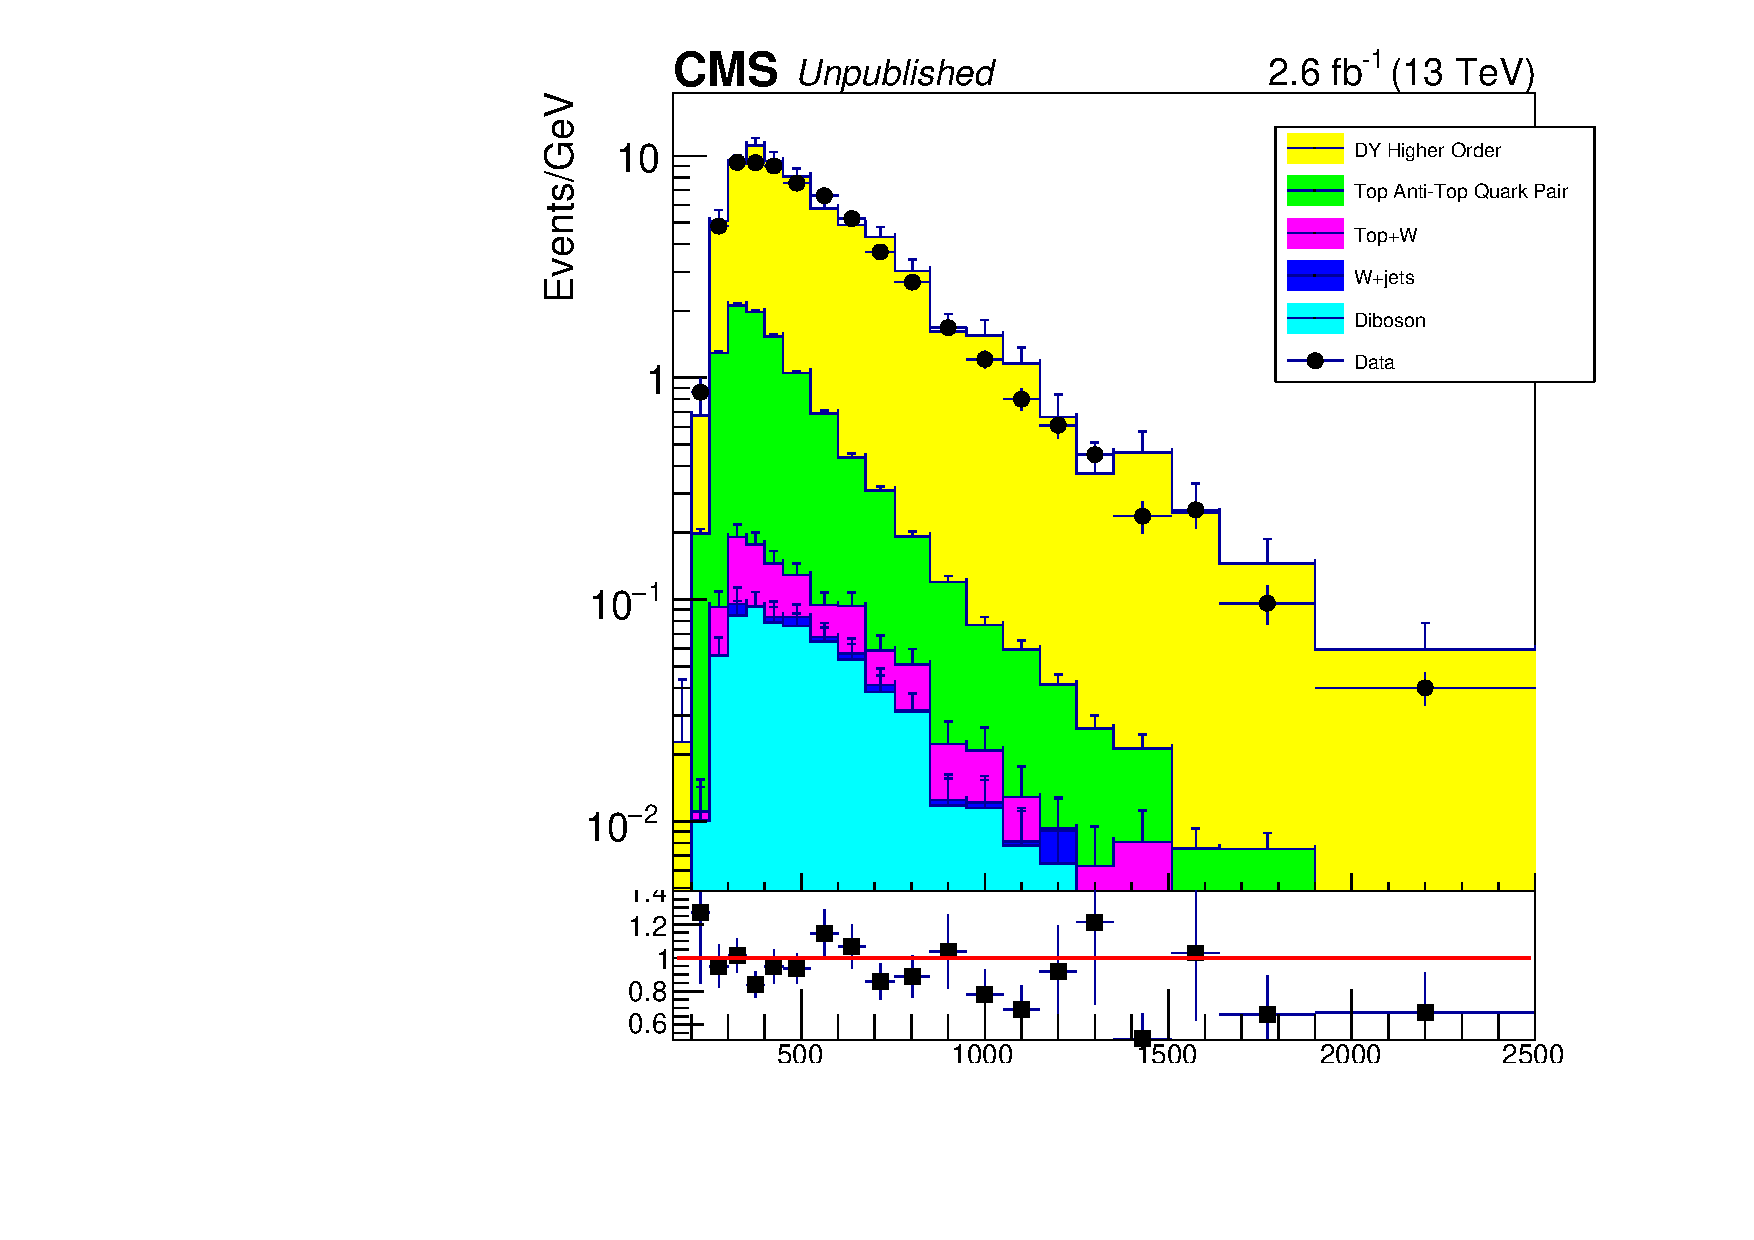
\includegraphics[width=0.45\textwidth]{figures/Mlljj_eeChnl_lowMllCR_AMCNLO.pdf}
}
\subfigure{
  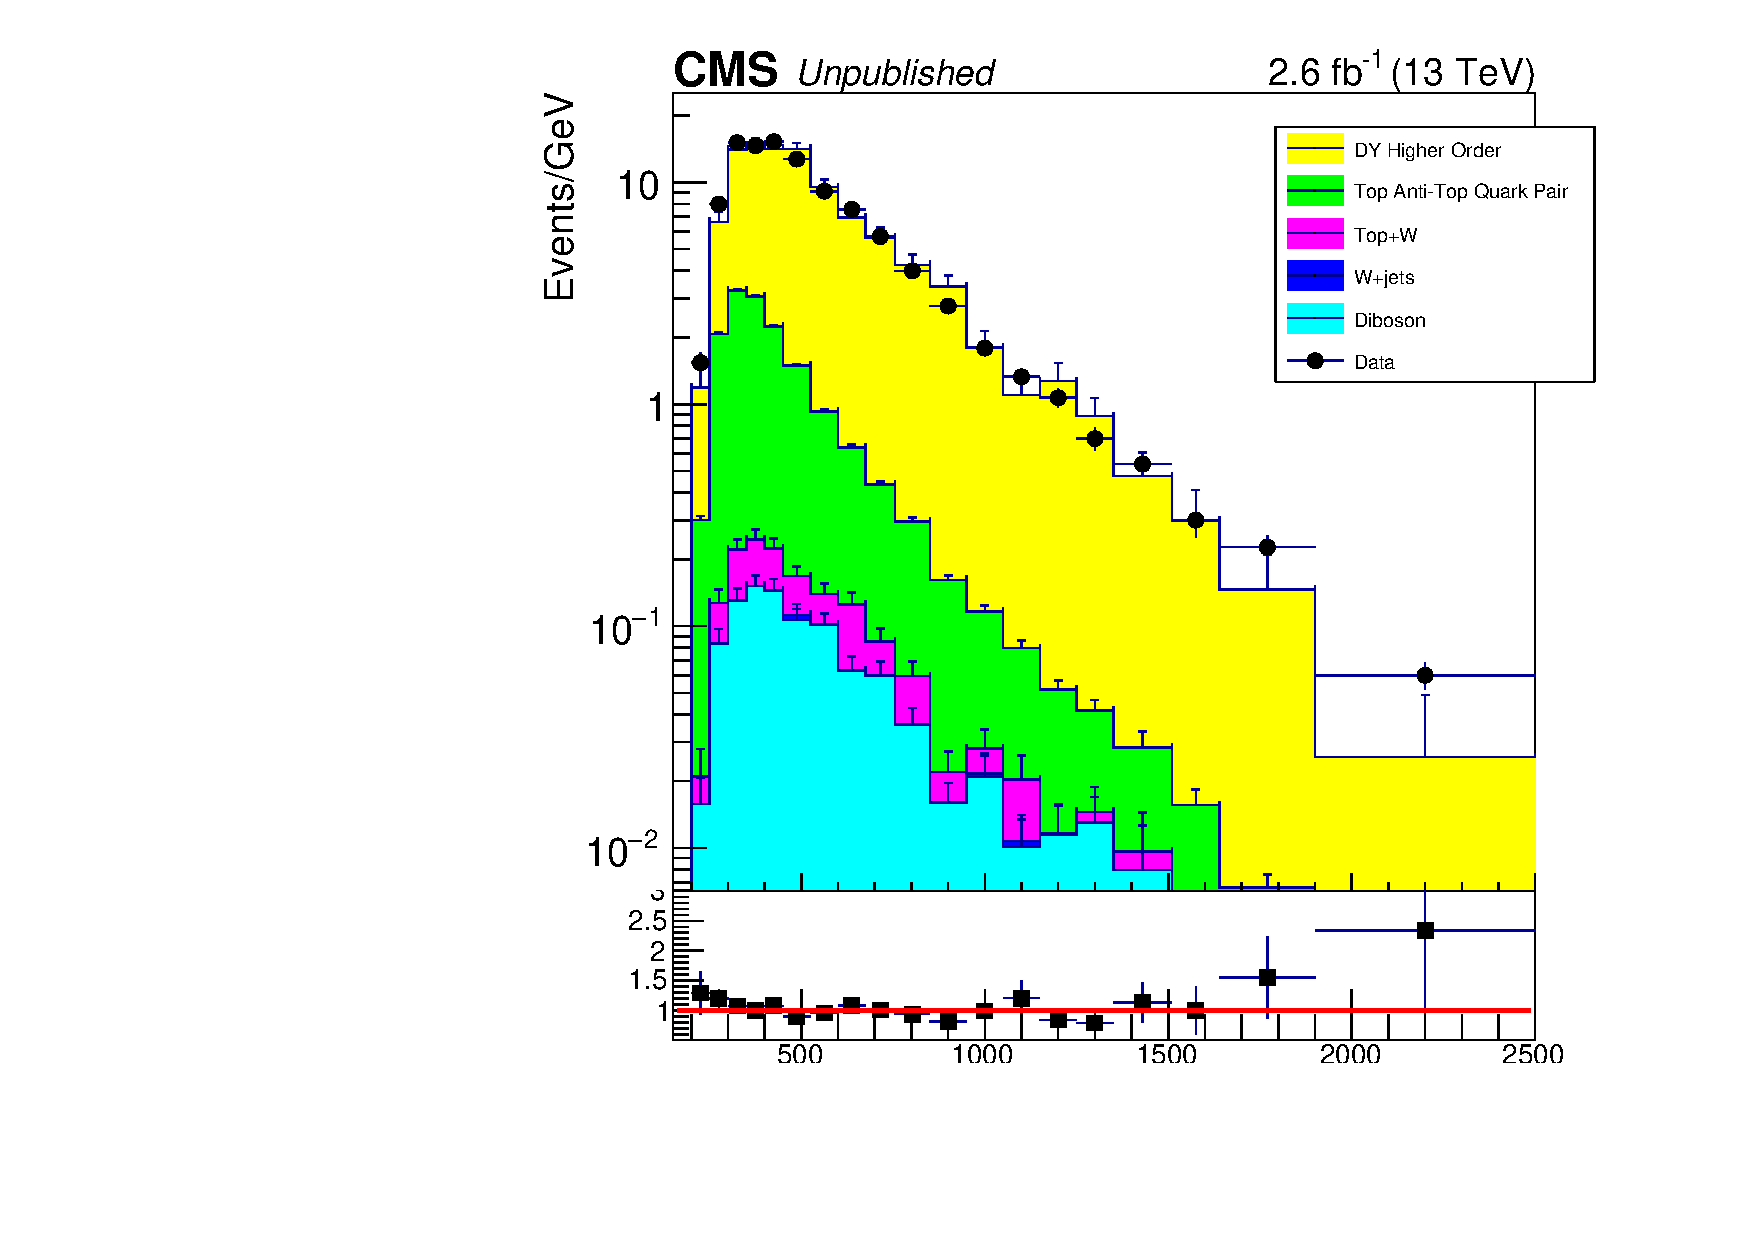
\includegraphics[width=0.45\textwidth]{figures/Mlljj_mumuChnl_lowMllCR_AMCNLO.pdf}
}
\caption{The $\Mlljj$ distribution found in data and simulated background events that passed the $\Mll < 180 \GeV$ selection criteria.  The 
		$ee$-channel is on the left, and the $\mu\mu$-channel is on the right.  The bin contents are normalized to their widths.}
\label{fig:mlljjLowMllCRAMC}
\end{figure}

The low $\Mlljj$ control region was used to validate the $\sim$15\% correction applied, and 40\% uncertainty assigned to the estimated 
\DY normalization.  Events from data and all background simulations were selected using the same selection criteria as the low $\Mll$ 
control region, but with $\Mll > 200$ $\GeV$ and $\Mlljj < 600$ $\GeV$.  The weight of \DY events was increased by $\sim$15\%, and then 
the $\Mll$ distributions found in selected data and simulated background events were compared.  The comparison, shown in Figure 
\ref{fig:mllInLowMlljjSideband}, showed that the $\sim$15\% \DY correction brought the background estimate into better agreement with the 
data.  In addition, the 40\% \DY normalization uncertainty was not too conservative, because the disagreement between data and estimated 
backgrounds approached 40\% in several bins.

\begin{figure}[btp]
\centering
\subfigure{
  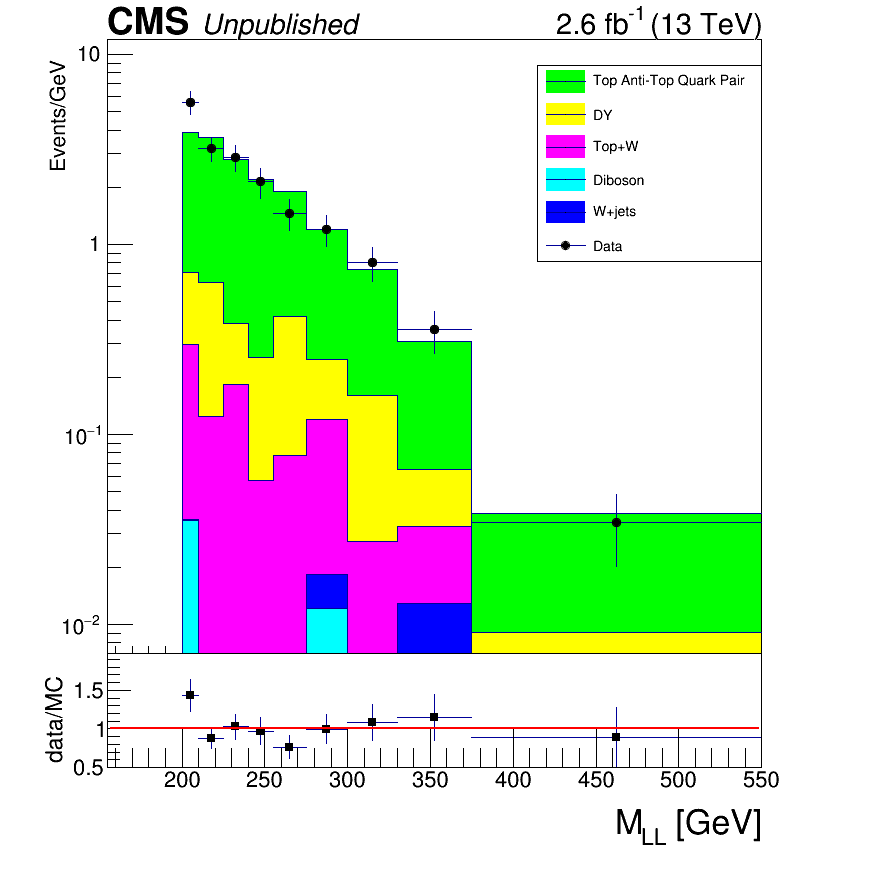
\includegraphics[width=0.45\textwidth]{figures/Mll_eeChnl_lowMlljjCR.png}
}
\subfigure{
  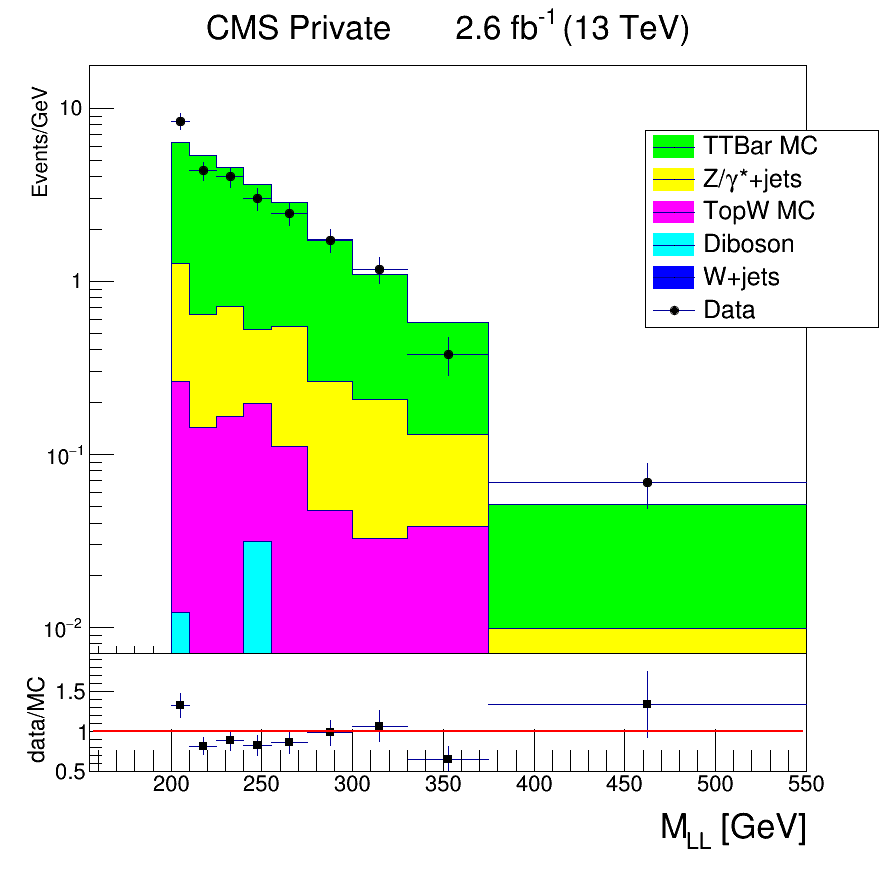
\includegraphics[width=0.45\textwidth]{figures/Mll_mumuChnl_lowMlljjCR.png}
}
\caption{The $\Mll$ distribution found in data and simulated background events that passed the low $\Mlljj$ control region requirements.  
The $ee$-channel is on the left, and the $\mu\mu$-channel is on the right.}
\label{fig:mllInLowMlljjSideband}
\end{figure}

\subsection{\DY Background Summary}
The \DY contribution to the $\Mlljj$ distribution found in data was estimated by selecting simulated \DY events using the selection criteria 
described in Chapter \ref{sec:reco_chapter}.  The weight of each selected event was increased by 15.7\% the $ee$-channel, and by 14.2\% in 
the $\mu\mu$-channel.  When the search results were calculated, a 40\% uncertainty was assigned to the estimated number of \DY events.


\section{Diboson and W+jets Backgrounds}
\label{sec:dibosonAndWJetsBkgnds}
%The $\DY$+jets interaction produced $\ell\ell jj$ events at a similar rate to the top quark interactions.  The $\Mlljj$ distribution 
%produced by the \DY+jets interaction was estimated using simulated \DY+jets events.  Simulated \DY+jets events were selected using 
%the $ee$- and $\mu\mu$-channel requirements.  Selected events defined the shape of the $\Mlljj$ distribution in both channels, but 
%the magnitude was adjusted based on comparisons between simulations and data in three control regions.
The diboson (WW, WZ, ZZ) and W+jets interactions produced $\ell\ell jj$ events at a much lower rate than the $\DY$+jets interaction.  In 
addition, no control region existed where diboson or W+jets interactions produced the dominant background.  Thus the shapes and magnitudes 
of the diboson and W+jets $\Mlljj$ distributions were estimated directly from simulated events, which were selected using the selection 
criteria described in Chapter \ref{sec:reco_chapter}.  The $\Mlljj$ distribution found in selected diboson and W+jets events (Figure 
\ref{fig:allExpectedBkgnds}) was concentrated in the $\Mlljj \leq 2.0$ $\TeV$ region, and its integral was less than 3\% of the predicted 
$\DY$+jets $\plus$ top quark background events.  For these reasons the diboson and W+jets contributions to the $\Mlljj$ distribution found 
in data were neglected.

\begin{figure}[h]
	\centering
	\subfigure{
		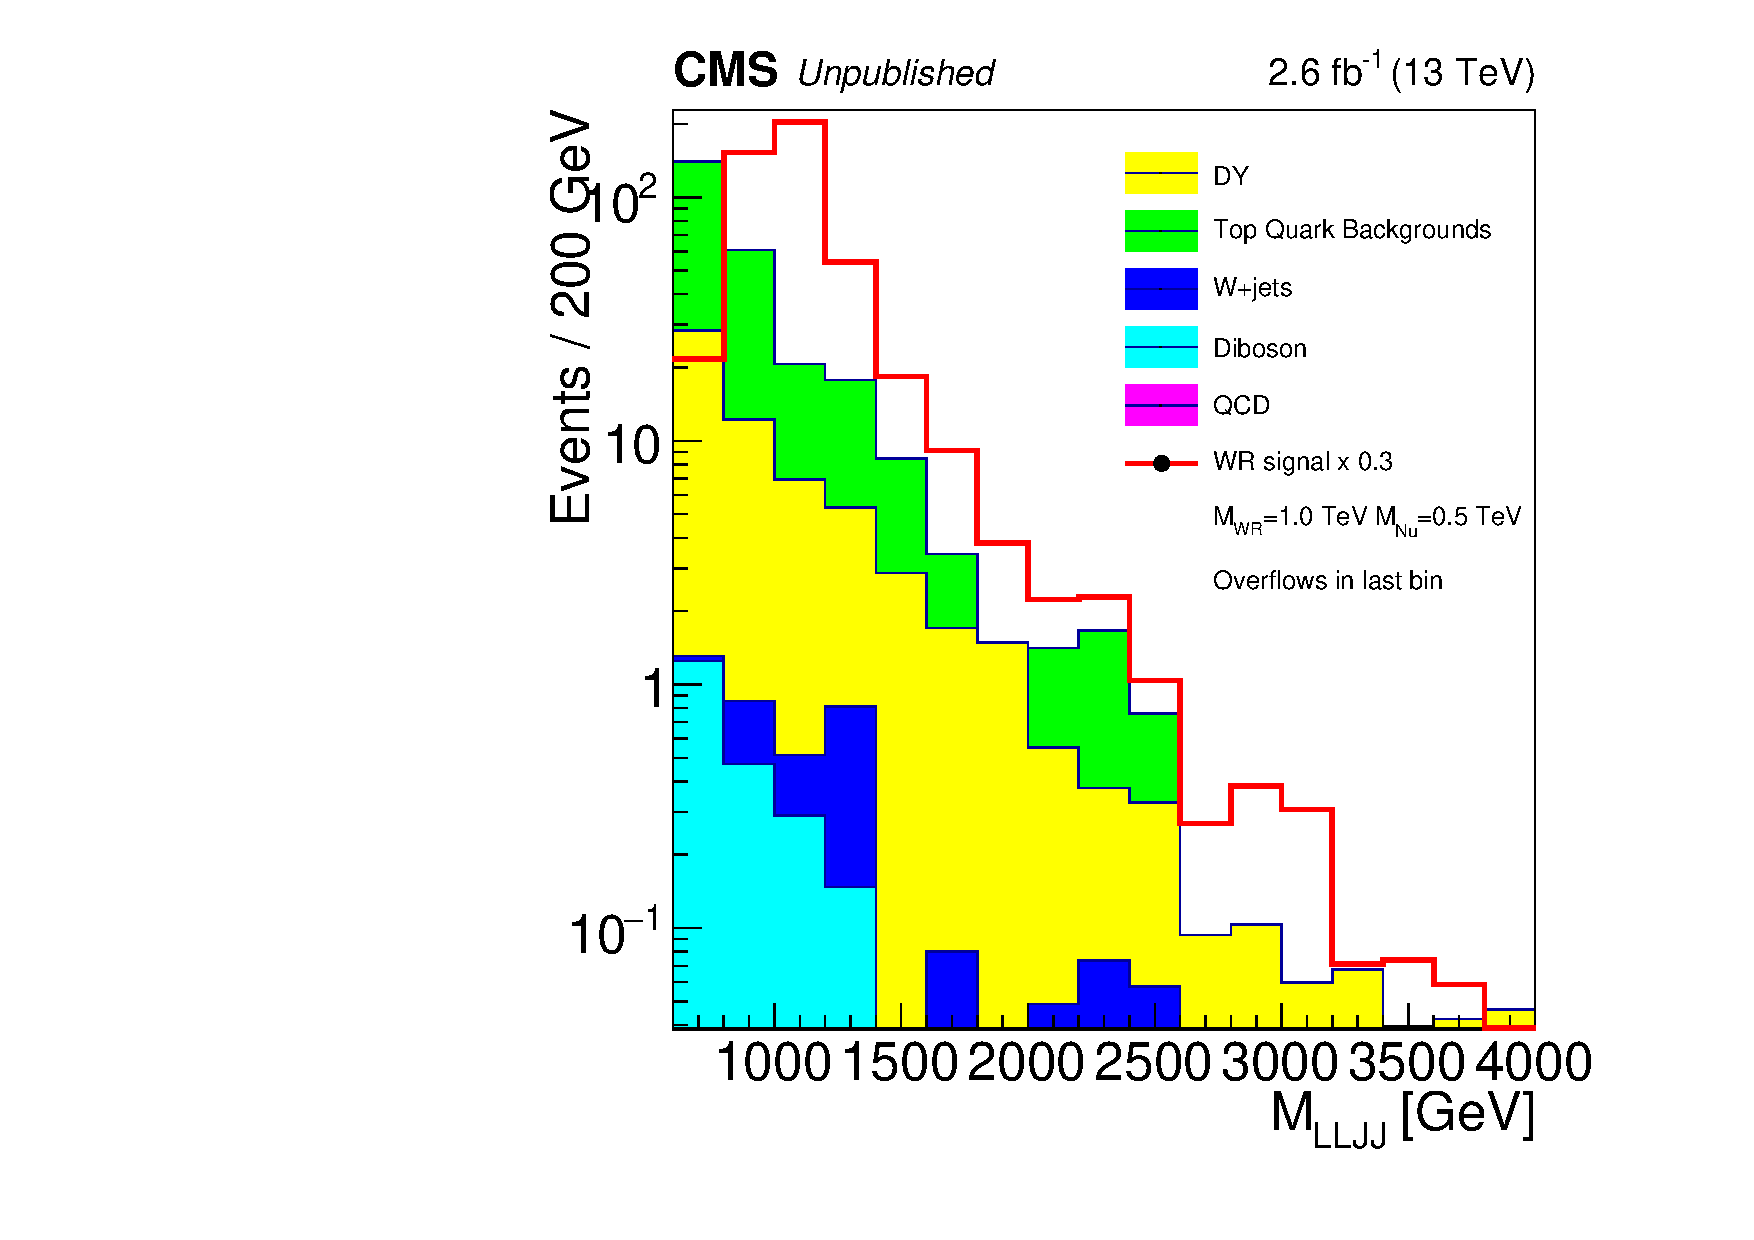
\includegraphics[width=0.45\textwidth]{figures/useOfLLJJMassAsFigureOfMerit.pdf}
	}
	\subfigure{
		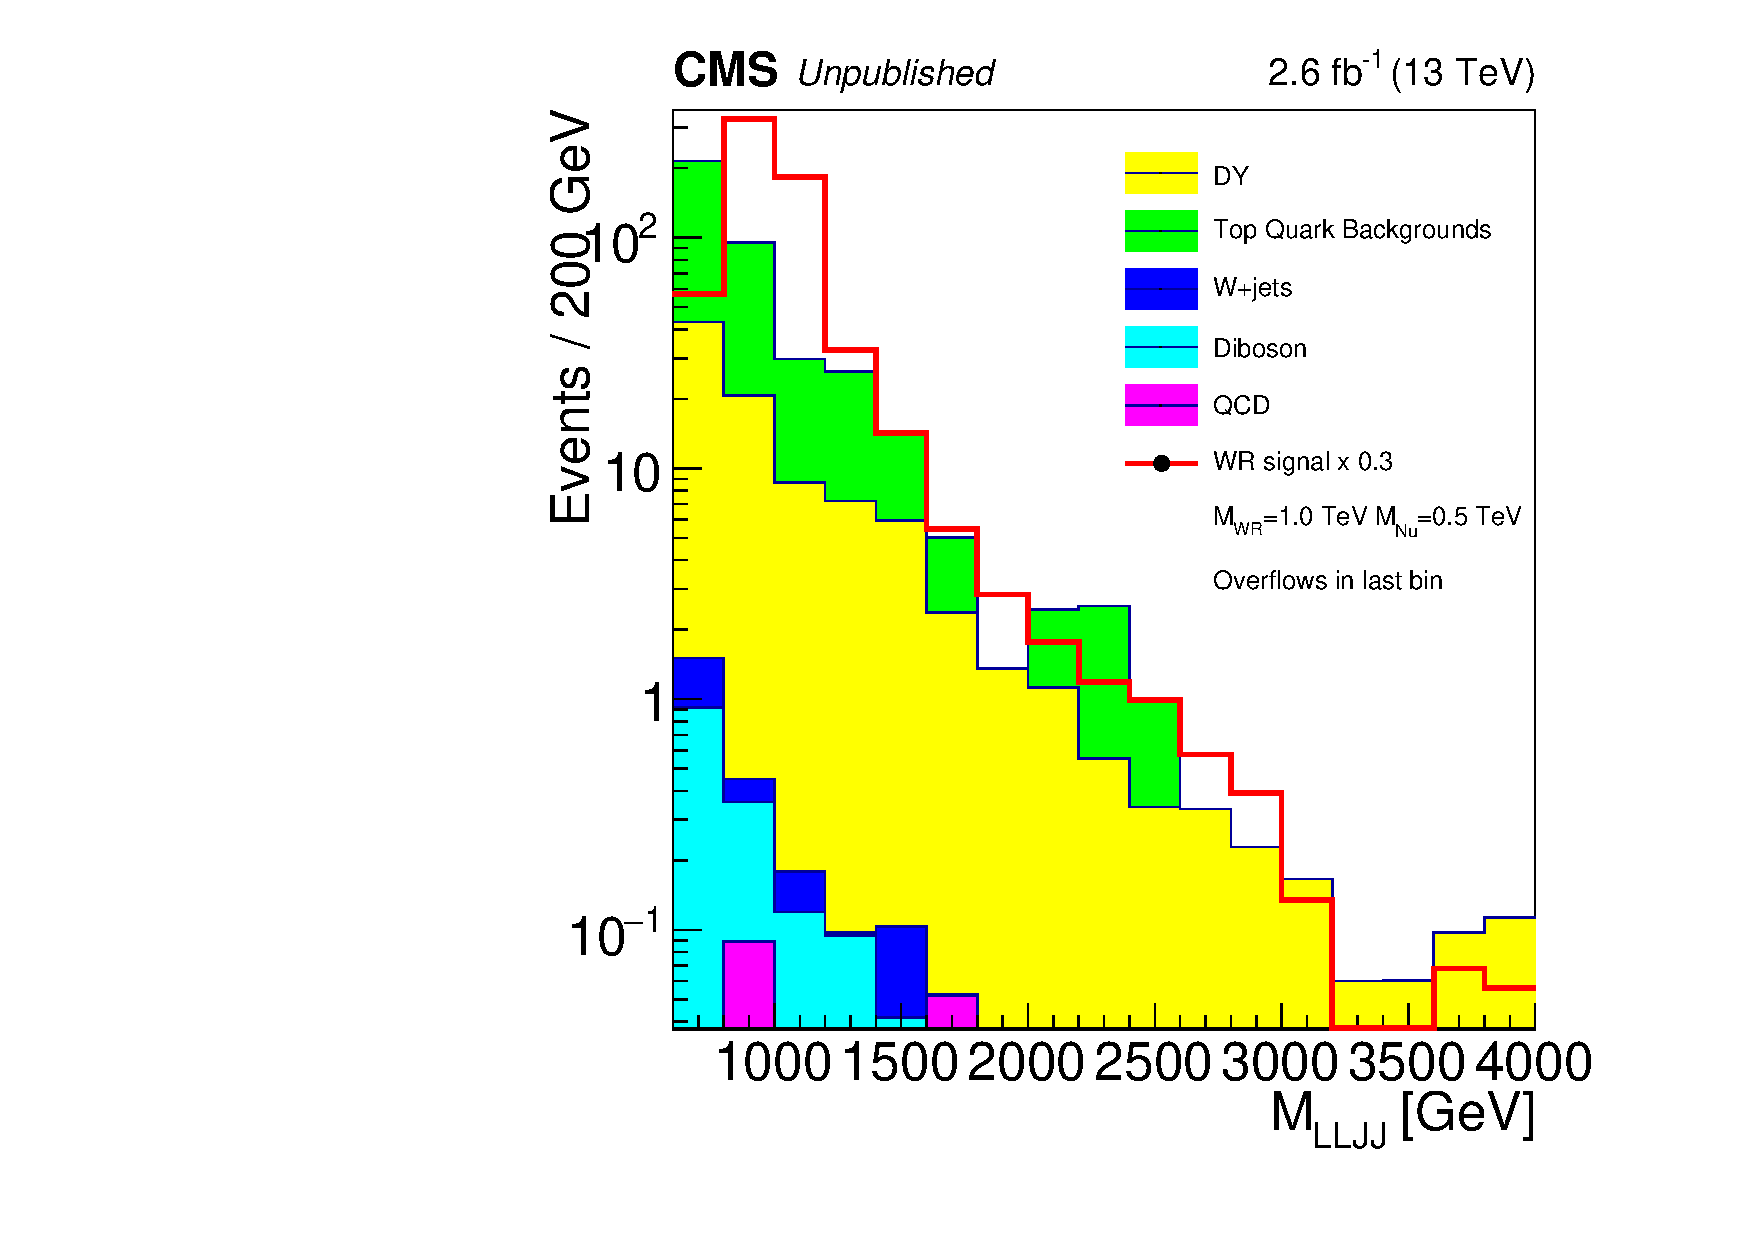
\includegraphics[width=0.45\textwidth]{figures/Mlljj_mumuChnl_signalRegionNoData.pdf}
	}
	\label{fig:allExpectedBkgnds}
	\caption{The $\Mlljj$ distributions found in selected \WR, \DY, diboson, W+jets, top quark, and QCD events.  The top quark and QCD 
		background distributions were extracted from the data. The \WR $\Mlljj$ distribution normalization was reduced by 70\% to compare 
		the shape of the signal and background distributions.  The $ee$-channel is on the left, and the $\mu\mu$-channel is on the right.}
\end{figure}


\section{QCD Background}
\label{sec:qcdBkgnd}
QCD multi-jet production yielded events where two charged leptons and jets were reconstructed.  In those events, two real 
jets were incorrectly reconstructed and identified as charged leptons.  The QCD multi-jet contribution to the $\Mlljj$ 
distribution found in data was estimated by selecting events in data with loose lepton ID requirements, then weighting selected 
events by the probability for selected leptons to pass the default (tight) lepton ID reuiqrements.  Data events were selected 
with the requirements described in Chapter \ref{sec:event_selection_chapter}, but with the following (looser) lepton ID 
requirements:

%RESUME HERE

\textbf{Muons}
\begin{itemize}
	\item The silicon tracker track was reconstructed from at least 1 hit in the silicon pixel detector, and at least 5 hits in the 
		entire tracker.
	\item The fitted track representing the estimated muon trajectory through all of CMS originated at a 
		point that was within 2 (5) mm of the muon's reconstructed vertex in the $x-y$ plane ($z$ axis). 
\end{itemize}

\textbf{Electrons}
\begin{itemize}
	\item At least 90\% of the SC energy was measured in a region 2 crystals wide in $\eta$.
	\item The ratio of hadronic energy in the HCAL tower behind the SC to the SC energy was $< 0.15$ 
		in the barrel, and $< 0.10$ in the endcap.
	\item The electron track missed 1 or fewer layers in the silicon pixel or inner silicon strip detectors.
	\item The electron track origin and its reconstructed vertex were separated by a small distance in the $x-y$ plane, 
		$\Delta_{xy} < 0.2$ mm in the tracker barrel, and $\Delta_{xy} < 0.5$ mm in the tracker endcap.
\end{itemize}

Events were not selected if one or more reconstructed leptons passed the default (tighter) lepton ID selections, as these 
events likely had one or more real leptons.  In selected events, the $\Et$ or $\pt$, and $\eta$ of the two selected leptons 
were used to calculate a probability for both leptons to pass the default lepton ID selections.  The probability was calculated 
using empirical formulas for electrons and muons derived from data, and each selected event was weighted by its probability.  
The contribution of weighted events, representing the QCD background, to the $\Mlljj$ distribution found in data is shown in 
Figure \ref{fig:allExpectedBkgnds}, and was negligible compared to other ST backgrounds.  Based on its small contribution, the 
QCD background was ignored when calculating results.


%%%%%%%%%%%%%%%%%%%%%%%%%%%%%%%%%%%%%%%%%%%%%%%%%%%%%%%%%%%%%%%%%%%%%%%%%%%%%%%%
